\chapter{IC}\label{sec:IC}
\section{Initial Conditions}

\subsection{Orbit integration}:

The orbit of the LMC is integrated backwards analiticaly:

The initial condition for all the orbits is the actual position 
$(X, Y, Z) = (-1, -41, -28)kpc$ and $(vx, vy, vz) = (-57, -226, 221)km/s$

\begin{table}[H]
\begin{center}
\begin{tabular}{c c c c c c c}
\hline
Model & x(kpc) & y(kpc) & z(kpc) &vx(km/s) & vy(km/s) & vz(km/s)\\
\hline
model1 & 40.8 & 241.7 & -89.68  & -17.31 & -156.68 & -8.76 \\
model2 & 40.4 & 243.46 & -84.75 & -17.45 & -161.62 & -12.02 \\
model3 & 39.75 & 245.96 & -77.89 & -17.59 & -168.41 & -16.84 \\     
model4 & 39.28 & 247.32 & -73.32 & -17.61 & -172.55 & -20.25 \\
model5 & 37.77 & 251.57 & -58.65 & -17.69 & -187.15 & -32.25 \\ 
model6 & 36.47 & 254.04 & -47.05 & -17.41 & -197.12 & -42.85 \\
\hline
\end{tabular}
\end{center}
\end{table}


\begin{figure}[H]
\centering
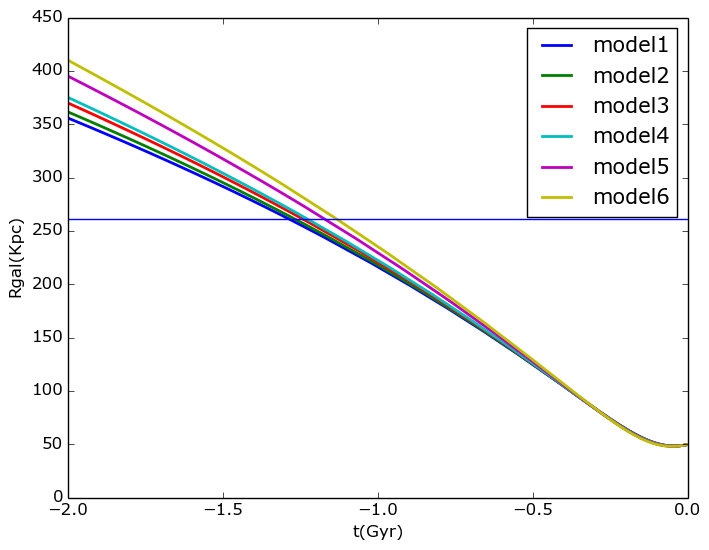
\includegraphics[scale=0.7]{../code/LMC_orbit/LMC_orbits.png}
\end{figure}
